\chapter{कण भौतिकी}\label{ch:b3:particle-physics}

% Provenance (not for print): second half of the "physique subatomique"
% module common to the surveyed third-year curricula: standard model
% inventory, interactions, conservation laws, detectors.

पदार्थ से उसकी संरचना परत-दर-परत छीलिए --- अणु, परमाणु,
नाभिक, न्यूक्लिऑन --- और वह छिलाई अचानक एक छोटी सूची पर रुक जाती है:
छह \emph{\omterm{def:b3:particle-physics:zoo}{क्वार्क}}, छह \emph{\omterm{def:b3:particle-physics:zoo}{लेप्टॉन}}, मुट्ठी भर बल-वाहक,
और 2012 में मिला एक शरमीला अदिश। आपने आज तक जो कुछ छुआ है, वह उस सूची
की तीन प्रविष्टियाँ हैं; और बाकी ब्रह्मांड के पहले माइक्रोसेकंड में
जिए थे और वहीं-वहीं फिर से, थोड़ी देर को, जीते हैं जहाँ
$E = mc^2$ पूरा चुका दिया जाए --- यानी ब्रह्मांडीय-किरणों के संघट्टों
और त्वरक-वलयों में। यह अध्याय सूची बनाता है: वे कण, उन्हें हिलाने
वाली चार अन्योन्यक्रियाएँ, संरक्षण-नियम
(\cref{ch:b3:lagrangian-mechanics} की नोएदर धाराएँ, जो अब
अवपरमाणविक हिसाब चला रही हैं), और वे संसूचक जो यह सब चित्रित करते
हैं। और यह आपकी अपनी अटारी में समाप्त होता है, जहाँ आप दस किलोमीटर
ऊपर बने म्यूऑन गिनते हैं।

\section{सूची}

\begin{definition}[लेप्टॉन, क्वार्क, हैड्रॉन]\label{def:b3:particle-physics:zoo}
\index{लेप्टॉन}\index{क्वार्क}\index{हैड्रॉन}\index{बैरिऑन}\index{मेसॉन}\index{प्रतिकण}
पदार्थ की निर्माण-ईंटें चक्रण-$\tfrac12$ वाले फ़र्मिऑन हैं
(\cref{ch:b3:spin-two-level}, \cref{ch:b3:identical-particles}), जो
छह-छह के दो कुलों में हैं। \emph{लेप्टॉन} प्रबल बल अनुभव नहीं करते:
इलेक्ट्रॉन, म्यूऑन और टाउ (आवेश $-e$, और हर एक पिछले से भारी)
तथा उनके तीन न्यूट्रिनो --- लगभग द्रव्यमानहीन, लगभग
असंसूचनीय। \emph{क्वार्क} छह स्वादों में आते हैं --- अप, डाउन,
स्ट्रेंज, चार्म, बॉटम, टॉप --- जिनके आवेश $+\tfrac23e$ (u, c,
t) और $-\tfrac13e$ (d, s, b) हैं, और वे कभी अकेले नहीं दिखते:
\emph{परिबंधन} उन्हें \emph{हैड्रॉनों} में बाँध देता है --- यानी
तीन-क्वार्क वाले \emph{बैरिऑन} (प्रोटॉन $=$ u u d, न्यूट्रॉन $=$ u d d) और
क्वार्क--प्रतिक्वार्क वाले \emph{मेसॉन} (पायॉन, केऑन)। हर कण का कोई
\emph{प्रतिकण} होता है, जिसका द्रव्यमान वही और आवेश उलटे होते हैं
(\cref{exo:b3:particle-physics:8})। साधारण पदार्थ केवल
पहली पीढ़ी काम में लेता है --- u, d, e, $\nu_{\text{e}}$; और दोनों
भारी प्रतिलिपियाँ, जहाँ तक कोई जानता है, केवल द्रव्यमान में भिन्न
हैं। ``यह किसने मँगाया था?'' --- भौतिकी आज भी पूछती है।
\end{definition}

\begin{omfigure}
\begin{tikzpicture}[scale=0.98,
  cell/.style={draw, minimum width=1.28cm, minimum height=1.05cm,
    font=\scriptsize, align=center, inner sep=1pt}]
  % quarks (2x3)
  \foreach \i/\n/\m in {0/u/{$+\tfrac23$}, 1/c/{$+\tfrac23$}, 2/t/{$+\tfrac23$}}
    \node[cell, fill=omDef!18] at (1.4*\i,1.1) {\textbf{\n}\\\m};
  \foreach \i/\n/\m in {0/d/{$-\tfrac13$}, 1/s/{$-\tfrac13$}, 2/b/{$-\tfrac13$}}
    \node[cell, fill=omDef!18] at (1.4*\i,0) {\textbf{\n}\\\m};
  % leptons
  \foreach \i/\n in {0/{e}, 1/{$\mu$}, 2/{$\tau$}}
    \node[cell, fill=omExo!20] at (1.4*\i,-1.35) {\textbf{\n}\\$-1$};
  \foreach \i/\n in {0/{$\nu_{\text{e}}$}, 1/{$\nu_\mu$}, 2/{$\nu_\tau$}}
    \node[cell, fill=omExo!20] at (1.4*\i,-2.45) {\textbf{\n}\\$0$};
  % bosons
  \node[cell, fill=omThm!15] at (5.0,1.1) {\textbf{g}\\प्रबल};
  \node[cell, fill=omThm!15] at (5.0,0) {\textbf{$\gamma$}\\वि-चु};
  \node[cell, fill=omThm!15] at (5.0,-1.35) {\textbf{W, Z}\\दुर्बल};
  \node[cell, fill=omThm!15] at (6.5,1.1) {\textbf{H}\\हिग्स};
  % generation labels
  \node[font=\scriptsize, anchor=south] at (0,1.75) {पहली};
  \node[font=\scriptsize, anchor=south] at (1.4,1.75) {दूसरी};
  \node[font=\scriptsize, anchor=south] at (2.8,1.75) {तीसरी};
  \node[font=\scriptsize, anchor=south] at (5.75,1.75) {वाहक};
  \node[font=\scriptsize, rotate=90, anchor=south] at (-1.05,0.55) {क्वार्क};
  \node[font=\scriptsize, rotate=90, anchor=south] at (-1.05,-1.9) {लेप्टॉन};
\end{tikzpicture}

{\small मानक प्रतिरूप की नामावली ($e$ की इकाइयों में आवेश)। उसका एक
स्तंभ हर परमाणु गढ़ता है; और बाकी दो महँगी
प्रतिध्वनियाँ हैं। गुरुत्व, जो इन द्रव्यमानों पर नाप से परे दुर्बल
है, इस मेज़ पर कोई कुर्सी नहीं रखता --- प्रतिरूप की सबसे प्रसिद्ध
रिक्ति।}
\end{omfigure}

\begin{remark}[चार अन्योन्यक्रियाएँ]\label{rem:b3:particle-physics:forces}
\index{प्रबल अन्योन्यक्रिया}\index{दुर्बल अन्योन्यक्रिया}\index{विद्युत्दुर्बल}
हर प्रक्रिया चार बलों में से किसी एक का काम है, और हर बल अपने
बोसॉन से ढोया जाता है। \emph{प्रबल} बल (ग्लूऑन) क्वार्कों को ऐसे
विभव से पकड़ता है जो दूरी के साथ \emph{बढ़ता} है --- दो क्वार्कों को
खींचकर अलग कीजिए और वह तना हुआ क्षेत्र टूटकर एक ताज़ा
क्वार्क--प्रतिक्वार्क युग्म बना देता है (\cref{exo:b3:particle-physics:1}): यही
परिबंधन है, और उसका अवशेष नाभिकों को जोड़े रखता है
(\cref{ch:b3:nuclear-physics})। \emph{विद्युत्-चुंबकत्व} (फ़ोटॉन,
द्रव्यमानहीन: अनंत परास) रसायन और प्रकाश चलाता है। और
\emph{दुर्बल} बल (W तथा Z, जो भारी हैं,
$\approx80$--$\qty{91}{GeV}$: परास $10^{-3}\,\unit{fm}$,
और इसीलिए ``दुर्बल'') अकेला स्वाद-बदलू है --- $\beta$ क्षय दरअसल
किसी d \omterm{def:b3:particle-physics:zoo}{क्वार्क} का u बन जाना है
(\cref{prop:b3:particle-physics:conservation}) --- और वही अकेला
बल है जिसका उत्तर न्यूट्रिनो देते हैं। \emph{गुरुत्व} दो प्रोटॉनों के
बीच विद्युत्-चुंबकत्व से $10^{36}$ गुना दुर्बल है और प्रयोगशाला में
उसकी कोई भूमिका नहीं --- फिर भी, अपरिरक्षित और लंबी-परास होने के
कारण, वही पूरा \cref{ch:b3:astrophysics} चलाएगा। विद्युत्-चुंबकत्व
और दुर्बल बल ऊँची ऊर्जा पर एक ही \emph{विद्युत्दुर्बल}
अन्योन्यक्रिया में एक हो जाते हैं --- और हमारी ठंडी ऊर्जाओं पर उन्हें
हिग्स क्षेत्र का \omterm{def:b3:phase-transitions:order}{सममिति-भंग} अलग करता है (\cref{exo:b3:particle-physics:9})।
\end{remark}

\section{हिसाब-किताब: संरक्षण-नियम}

\begin{proposition}[कण-अभिक्रियाओं के संरक्षण-नियम]\label{prop:b3:particle-physics:conservation}
\index{बैरिऑन संख्या}\index{लेप्टॉन संख्या}\index{संरक्षण-नियम!कण}
कोई अभिक्रिया तभी होती है जब बहीखाता बराबर बैठे। सदा
संरक्षित: ऊर्जा--संवेग
(\cref{ch:b3:relativistic-dynamics}), कोणीय संवेग, और
विद्युत् आवेश --- और हर एक की ज़मानत नोएदर की प्रमेय
(\cref{thm:b3:lagrangian-mechanics:noether}) देती है।
अब तक देखी गई हर अभिक्रिया में संरक्षित: \emph{\omterm{prop:b3:particle-physics:conservation}{बैरिऑन संख्या}}
$B$ (\omterm{def:b3:particle-physics:zoo}{बैरिऑन} $+1$, प्रति-बैरिऑन $-1$) और \emph{\omterm{prop:b3:particle-physics:conservation}{लेप्टॉन संख्या}}
$L$ (प्रति कुल, और वह भी बढ़िया परिशुद्धि से)। अतः प्रोटॉन, जो सबसे
हलका \omterm{def:b3:particle-physics:zoo}{बैरिऑन} है, क्षय के लिए कहीं जा ही नहीं सकता --- पदार्थ का
स्थायित्व एक हिसाब की प्रमेय है --- और $\beta$ क्षय को कोई
प्रति-न्यूट्रिनो भेजना ही पड़ता है:
\[
\text{n} \;\to\; \text{p} + \text{e}^- + \bar\nu_{\text{e}}
\qquad (\text{क्वार्क स्तर: } \text{d} \to \text{u} +
\text{e}^- + \bar\nu_{\text{e}}) ,
\]
जो $L$ को बराबर रखता है (और इलेक्ट्रॉन का सतत ऊर्जा-वर्णक्रम भी
समझा देता है, जिसने ऊर्जा-संरक्षण में भौतिकी का विश्वास
लगभग तोड़ ही दिया था, इससे पहले कि पाउली ने उसे बचाने के लिए
न्यूट्रिनो गढ़ लिया)।
स्वाद (विचित्रता, चार्म) प्रबल तथा
विद्युत्-चुंबकीय प्रक्रियाओं में संरक्षित रहते हैं पर \emph{दुर्बल
उन्हें तोड़ देता है}: विचित्र
कण भारी संख्या में जोड़ों में जन्मते हैं, फिर धीरे-धीरे और अकेले मरते
हैं --- और $10^{13}$ का वह अंतर, जो $\qty{e-23}{s}$ वाले प्रबल
जीवनकालों और $\qty{e-10}{s}$ वाले दुर्बल जीवनकालों के बीच है, ही
वह उँगली-छाप है जो बताती है कि उस क्षय पर किस बल ने दस्तख़त किए।
\end{proposition}
\admitted

\begin{omfigure}
\begin{tikzpicture}[scale=1.0]
  % neutron -> proton beta decay quark diagram
  % three quark lines left to right
  \draw[omDef, thick] (0,2.0) -- (7.2,2.0);
  \draw[omDef, thick] (0,1.45) -- (7.2,1.45);
  \draw[omDef, thick] (0,0.9) -- (3.3,0.9);
  \draw[omThm, thick] (3.3,0.9) -- (7.2,0.9);
  \node[omDef, font=\scriptsize, anchor=east] at (-0.1,2.0) {u};
  \node[omDef, font=\scriptsize, anchor=east] at (-0.1,1.45) {d};
  \node[omDef, font=\scriptsize, anchor=east] at (-0.1,0.9) {d};
  \node[omThm, font=\scriptsize, anchor=west] at (7.3,0.9) {u};
  \node[font=\scriptsize, anchor=west] at (7.3,1.45) {d};
  \node[font=\scriptsize, anchor=west] at (7.3,2.0) {u};
  % W boson wavy-ish (zigzag)
  \draw[omExo, thick] (3.3,0.9)
    -- (3.75,0.55) -- (4.05,0.75) -- (4.35,0.35) -- (4.65,0.55)
    -- (4.95,0.15) -- (5.25,0.35) -- (5.55,-0.05);
  \node[omExo, font=\scriptsize, anchor=west] at (4.75,0.72) {W$^-$};
  % electron and antineutrino
  \draw[thick] (5.55,-0.05) -- (7.2,0.25);
  \draw[thick] (5.55,-0.05) -- (7.2,-0.55);
  \node[font=\scriptsize, anchor=west] at (7.3,0.25) {e$^-$};
  \node[font=\scriptsize, anchor=west] at (7.3,-0.55) {$\bar\nu_{\text{e}}$};
  % braces labels
  \node[font=\scriptsize, anchor=east] at (-0.75,1.45) {न्यूट्रॉन};
  \node[font=\scriptsize, anchor=west] at (8.35,1.45) {प्रोटॉन};
\end{tikzpicture}

{\small $\beta$ क्षय, \omterm{def:b3:particle-physics:zoo}{क्वार्क} स्तर तक ज़ूम किया हुआ: कोई एक d \omterm{def:b3:particle-physics:zoo}{क्वार्क}
किसी आभासी W$^-$ को उत्सर्जित करके u बन जाता है, और वह W
इलेक्ट्रॉन तथा प्रति-न्यूट्रिनो के रूप में साकार हो जाता है। हर
बहीखाता बराबर बैठता है: आवेश
$-\tfrac13 = +\tfrac23 - 1 + 0$, \omterm{prop:b3:particle-physics:conservation}{बैरिऑन संख्या}, \omterm{prop:b3:particle-physics:conservation}{लेप्टॉन संख्या}।}
\end{omfigure}

\section{कण बनाना और देखना}

\begin{remark}[त्वरक और संसूचक]\label{rem:b3:particle-physics:machines}
\index{संघट्टक}\index{कण संसूचक}
त्वरित करने के दो कारण: \emph{वियोजन} --- कोई जाँच-कण अपनी
तरंगदैर्घ्य $\lambda = h/p$ से महीन ब्योरा नहीं देखता
(\cref{ch:b3:crystalline-solids} ने आंगस्ट्रॉम काम में लिए थे;
फ़ेम्टोमीटर \unit{GeV}s माँगते हैं) --- और \emph{सृजन}: संघट्ट की
ऊर्जा नया द्रव्यमान बन जाती है, और दो पुंजों को सम्मुख टकराना उसे
पूरा का पूरा खर्च कर देता है (जबकि कोई स्थिर लक्ष्य उसका अधिकांश
मलबे को आगे ढोने में गँवा देता है:
\cref{exo:b3:particle-physics:4})। वृत्ताकार संघट्टक उन्हीं कणों को
उसी त्वरक-अंतराल से बार-बार गुज़ारते हैं जबकि चुंबक उन्हें मोड़ते
रहते हैं --- और इसकी क़ीमत सिंक्रोट्रॉन विकिरण
$\propto\gamma^4$ है, और इसीलिए जिस वलय ने हिग्स पाया वह
भारी प्रोटॉन टकराता है, हलके-फुल्के इलेक्ट्रॉन नहीं। उस
कटान-बिंदु के चारों ओर प्याज़ की परतें बैठी हैं, और हर एक एक ही
प्रश्न पूछती है: कोई \emph{अनुरेखक} आवेशित पथों को किसी चुंबक में
मोड़ता है (संवेग); कोई विद्युत्-चुंबकीय \emph{कैलोरीमापी}
इलेक्ट्रॉन और फ़ोटॉन निगल जाता है (ऊर्जा); कोई हैड्रॉनी वाला
पायॉन और प्रोटॉन निगलता है; और केवल म्यूऑन ही सबसे बाहरी कक्षों तक
भेदकर पहुँचते हैं --- यानी दफ़्न की गहराई से पहचान। न्यूट्रिनो
लापता संवेग के रूप में निकल जाते हैं: और बहीखाता उसे संसूचित कर लेता
है जिसे कोई रोक नहीं सकता।
\end{remark}

\begin{omfigure}
\begin{tikzpicture}[scale=1.0]
  % quadrant onion detector
  \fill[omDef!10] (0,0) -- (4.7,0) arc (0:80:4.7) -- cycle;
  \fill[omExo!18] (0,0) -- (3.5,0) arc (0:80:3.5) -- cycle;
  \fill[omThm!12] (0,0) -- (2.3,0) arc (0:80:2.3) -- cycle;
  \fill[white] (0,0) -- (1.2,0) arc (0:80:1.2) -- cycle;
  \foreach \r in {1.2,2.3,3.5,4.7} \draw[gray] (\r,0) arc (0:80:\r);
  \draw[gray] (0,0) -- (4.7,0);
  \draw[gray] (0,0) -- (80:4.7);
  % labels of layers, along the free bottom edge
  \node[font=\tiny, anchor=north] at (1.75,-0.12) {अनुरेखक};
  \node[font=\tiny, anchor=north] at (2.9,-0.12) {वि-चु कैलोरीमापी};
  \node[font=\tiny, anchor=north] at (4.1,-0.12) {हैड्रॉनी कैलोरीमापी};
  \node[font=\tiny, anchor=west] at (12:4.85) {म्यूऑन कक्ष};
  % particle tracks from origin
  % electron: curved, stops in ecal
  \draw[omDef, thick] (0,0) .. controls (1.1,0.62) .. (2.05,1.55);
  \fill[omDef] (2.6,1.9) circle (2pt);
  \node[omDef, font=\tiny, anchor=south west] at (2.5,1.98) {e$^-$};
  % photon: straight dashed (neutral), stops in ecal
  \draw[omDef, dashed] (0,0) -- (55:2.75);
  \fill[omDef] (55:2.95) circle (2pt);
  \node[omDef, font=\tiny, anchor=south] at (55:3.2) {$\gamma$};
  % pion: curved into hadronic
  \draw[omThm, thick] (0,0) .. controls (0.75:2.0) and (5:2.6) .. (12:3.9);
  \fill[omThm] (14:4.1) circle (2pt);
  \node[omThm, font=\tiny, anchor=north] at (10:4.28) {$\pi$};
  % muon: nearly straight, exits
  \draw[omExo, very thick] (0,0) .. controls (70:2.4) .. (73:5.2);
  \node[omExo, font=\tiny, anchor=south] at (73:5.35) {$\mu$};
\end{tikzpicture}

{\small किसी संघट्टक-संसूचक का \omterm{def:b3:scattering-theory:cross-section}{अनुप्रस्थ काट}। हर जाति
अपना हस्ताक्षर लिखती है: आवेशित पगडंडियाँ अनुरेखक के क्षेत्र में मुड़
जाती हैं; इलेक्ट्रॉन और फ़ोटॉन भीतरी कैलोरीमापी में मरते हैं,
\omterm{def:b3:particle-physics:zoo}{हैड्रॉन} बाहरी में; केवल म्यूऑन ही दूर के कक्षों तक पहुँचते हैं; और
जो बिना दिखे भाग जाता है --- यानी न्यूट्रिनो --- वह लापता संवेग से
पढ़ लिया जाता है।}
\end{omfigure}

\begin{remark}[हिग्स, और खुला बहीखाता]\label{rem:b3:particle-physics:higgs}
\index{हिग्स बोसॉन}\index{कृष्ण पदार्थ}
मानक प्रतिरूप की सममिति उसके कणों के लिए नंगे द्रव्यमान वर्जित करती
है; और \emph{हिग्स क्षेत्र}, जो पूरी समष्टि को किसी अशून्य संघनित से
भर देता है --- अर्थात् \cref{ch:b3:phase-transitions} वाला
दोहरे-कूप का चुनाव, जो स्वयं निर्वात तक पदोन्नत हो गया ---
उस सममिति को भंग करता है और अपने युग्मनों के ज़रिए द्रव्यमान बाँटता
है: कण जितना भारी, पकड़ उतनी प्रबल। उसका अपना क्वांटम, यानी \omterm{rem:b3:particle-physics:higgs}{हिग्स
बोसॉन} (\qty{125}{GeV}, 2012 में मिला), उस मेज़ को पूरा कर गया। पर
खुला बहीखाता लंबा है: न्यूट्रिनो स्वादों के बीच दोलन करते हैं और
इसलिए उनका द्रव्यमान होना ही चाहिए, जो प्रतिरूप ने लिखा ही नहीं
(\cref{exo:b3:particle-physics:10}); आकाशगंगाएँ ऐसे घूमती हैं मानो
जितना चमकता है उससे पाँच गुना अधिक पदार्थ उन्हें थामे हो
(\cref{ch:b3:astrophysics}); और ब्रह्मांड में पदार्थ है
पर प्रतिपदार्थ लगभग नहीं, और इस असममिति की क़ीमत प्रतिरूप का नन्हा
CP-भंग अभी नहीं चुका सकता। यह सूची ही उस सबका पाठ्यक्रम है
जो आगे आना है।
\end{remark}

\begin{omfigure}
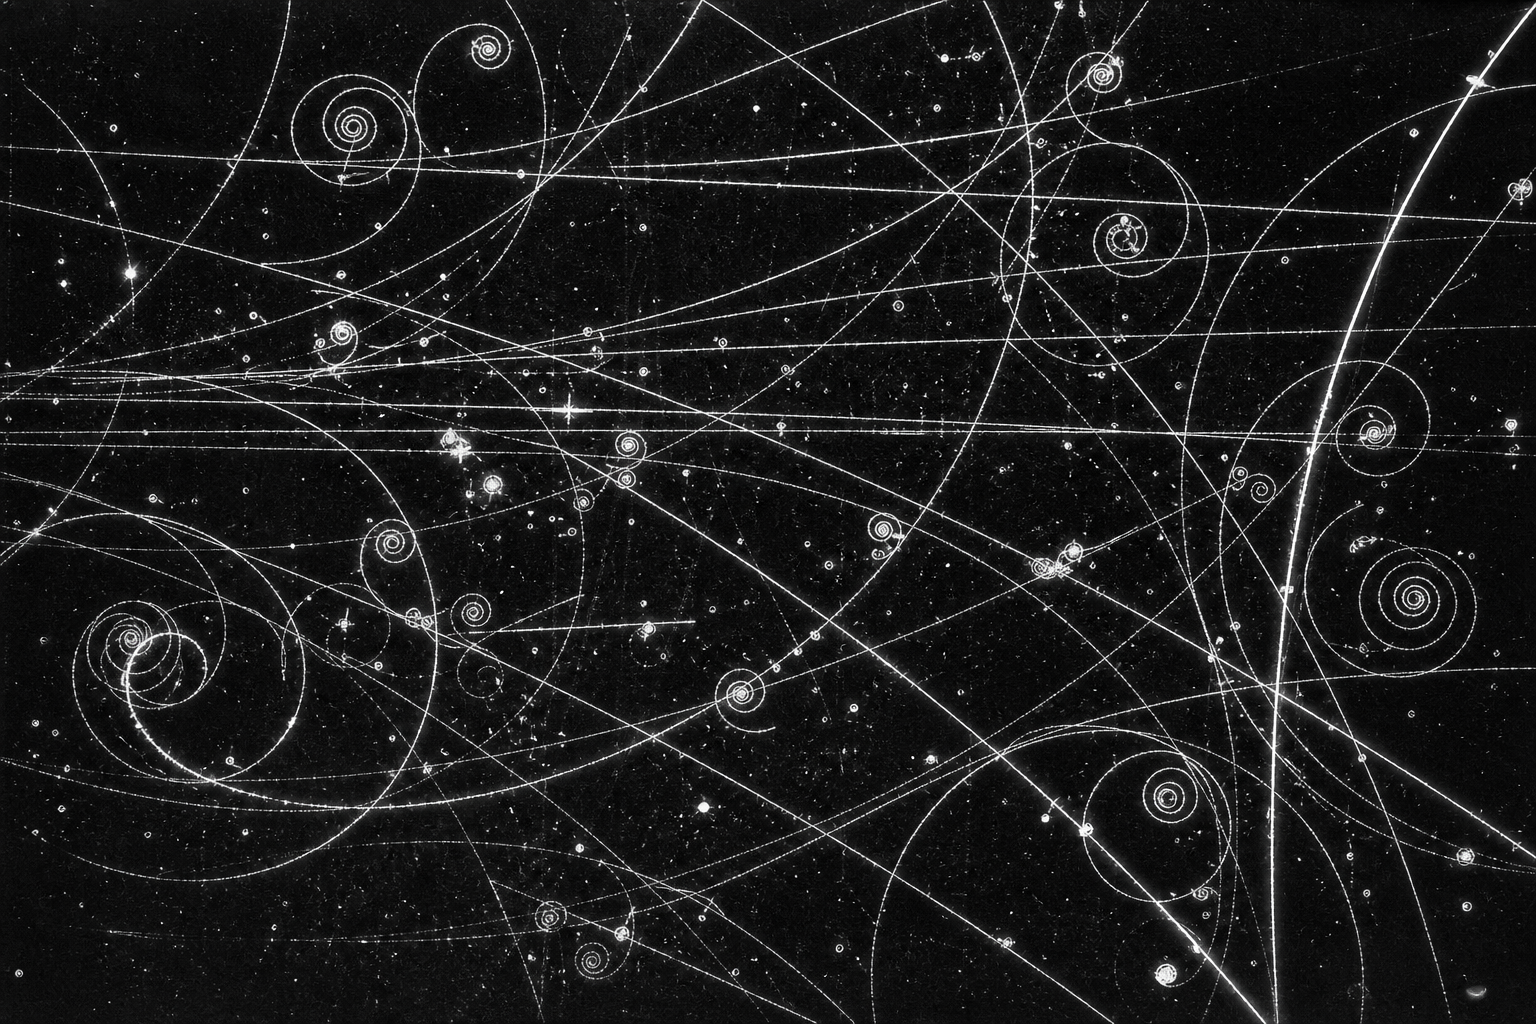
\includegraphics[width=0.58\linewidth]{images/book5/ai/b5-22-bubble-chamber-spirals.png}

{\small किसी बुलबुला-कक्ष का दृश्य: किसी चुंबकीय क्षेत्र में कुंडली मारती आवेशित पगडंडियाँ, और ऊर्जा खोते हुए उलटी-उलटी दिशाओं में सर्पिल बनाते इलेक्ट्रॉन तथा पॉज़िट्रॉन। दशकों तक कण भौतिकी ऐसी ही फ़िल्म से फ़्रेम-दर-फ़्रेम पढ़ी जाती रही।}
\end{omfigure}

\section{अभ्यास}

\begin{exercise}[$\star$]\label{exo:b3:particle-physics:1}
\omterm{def:b3:particle-physics:zoo}{क्वार्क} का अंकगणित। (क) p $=$ u u d और
n $=$ u d d के आवेश सत्यापित कीजिए। (ख) पायॉन $\pi^+$
$\text{u}\bar{\text{d}}$ है:
उसका आवेश जाँचिए। (ग) $\pi^-$ के लिए और
$\Delta^{++}$ (आवेश $+2e$) के लिए क्वार्क-संघटन सुझाइए। (घ) किसी
प्रोटॉन से कोई \omterm{def:b3:particle-physics:zoo}{क्वार्क} बाहर खींचने पर किसी मुक्त \omterm{def:b3:particle-physics:zoo}{क्वार्क} के बजाय
मेसॉनों की झड़ी क्यों मिलती है?
\end{exercise}

\begin{exercise}[$\star$]\label{exo:b3:particle-physics:2}
छँटाई। e$^-$, $\nu_\mu$, $\pi^+$, p, n,
$\mu^-$ में से हर एक के लिए: (क) \omterm{def:b3:particle-physics:zoo}{लेप्टॉन}, \omterm{def:b3:particle-physics:zoo}{बैरिऑन} या \omterm{def:b3:particle-physics:zoo}{मेसॉन}? (ख) कौन
प्रबल बल अनुभव करते हैं? (ग) कौन अकेले में स्थायी हैं? (घ) किसे कोई
चुंबकीय क्षेत्र विक्षेपित नहीं कर सकता?
\end{exercise}

\begin{exercise}[$\star$]\label{exo:b3:particle-physics:3}
अनुमत या वर्जित? फ़ैसला दीजिए, और यदि कोई नियम टूटता हो तो उसका नाम भी:
(क) $\text{n} \to \text{p} + \text{e}^- + \bar\nu_{\text{e}}$;
(ख) $\text{p} \to \text{n} + \text{e}^+ + \nu_{\text{e}}$ (किसी
\emph{मुक्त} प्रोटॉन के लिए);
(ग) $\text{p} \to \text{e}^+ + \gamma$;
(घ) $\mu^- \to \text{e}^- + \gamma$।
\end{exercise}

\begin{exercise}[$\star$]\label{exo:b3:particle-physics:4}
सृजन की क़ीमत। किसी हाइड्रोजन लक्ष्य पर किसी प्रोटॉन पुंज से
प्रोटॉन--प्रतिप्रोटॉन युग्म बनाने के लिए
(\cref{ch:b3:relativistic-dynamics} के निश्चर-द्रव्यमान तर्क से)
$6m_{\text{p}}c^2$ की पुंज-गतिज ऊर्जा चाहिए। (क) उसका मान GeV में निकालिए।
(ख) किसी संघट्टक में उसी युग्म के लिए कितनी गतिज ऊर्जा वाले दो पुंज
काफ़ी हैं? (ग) ``बरबादी'' का अनुपात निकालिए और समझाइए कि
स्थिर-लक्ष्य की ऊर्जा कहाँ जाती है। (घ) 1955 में प्रतिप्रोटॉन खोजने
वाली मशीन को $\sim\qty{6}{GeV}$ क्यों चाहिए थी?
\end{exercise}

\begin{exercise}[$\star\star$]\label{exo:b3:particle-physics:5}
म्यूऑन, दो-दो बार। म्यूऑन ($m = \qty{106}{MeV}$,
$\tau = \qty{2.2}{\micro s}$) इलेक्ट्रॉन का भारी जुड़वाँ है। (क)
$c\tau$ कितनी दूरी है? (ख) \qty{15}{km} पर जन्मे ब्रह्मांडीय
म्यूऑन ज़मीन तक पहुँच जाते हैं: जीवित रहने के लिए कितना $\gamma$
चाहिए, और वह कितनी ऊर्जा है? (ग) स्वयं म्यूऑन के तंत्र से वही
जीवित रहना बताइए। (घ) म्यूऑन इलेक्ट्रॉन में क्षय क्यों करता है और
किसी प्रोटॉन में कभी क्यों नहीं, और कण के मानकों से उसका क्षय
\emph{धीमा} क्यों है?
\end{exercise}

\begin{exercise}[$\star\star$]\label{exo:b3:particle-physics:6}
$\beta$ क्षय के भीतर। (क) न्यूट्रॉन का क्षय \omterm{def:b3:particle-physics:zoo}{क्वार्क}
स्तर पर लिखिए और सारी संरक्षित राशियाँ जाँचिए। (ख) उत्सर्जित
इलेक्ट्रॉन का ऊर्जा-वर्णक्रम किसी अंत-बिंदु तक सतत है:
समझाइए कि इसने कभी ऊर्जा-संरक्षण को कैसे ख़तरे में डाला और
पाउली के न्यूट्रिनो ने उसे कैसे बचाया। (ग) W बोसॉन का भार
\qty{80.4}{GeV} है: दुर्बल बल की परास
$\hbar/m_{\text{W}}c$ आकलिए ($\hbar c = \qty{197}{MeV.fm}$)। (घ) उस
परास से एक वाक्य में समझाइए कि ``दुर्बल'' बल कम ऊर्जा पर दुर्बल
क्यों है और ऊँची पर विद्युत्दुर्बल-प्रबल क्यों।
\end{exercise}

\begin{exercise}[$\star\star$]\label{exo:b3:particle-physics:7}
विचित्र हिसाब। केऑन और $\Lambda$ हाइपेरॉन एक स्वाद ढोते हैं,
यानी \emph{विचित्रता}, जो प्रबल बल से संरक्षित है पर
दुर्बल से नहीं। (क) समझाइए कि ब्रह्मांडीय-किरणों के संघट्ट विचित्र
कण केवल जोड़ों में क्यों पैदा करते हैं। (ख) $\Lambda$
$\qty{2.6e-10}{s}$ जीता है --- प्रबल क्षयों के $\qty{e-23}{s}$ से
तुलिए और निष्कर्ष निकालिए कि उसे कौन-सा बल मारता है। (ग) कौन-सा
काल-पैमाना-अनुपात दोनों को अलग करता है, और वह रोज़मर्रा के किस
अनुपात के तुल्य है (एक सेकंड बनाम क्या)? (घ) इस ``विचित्र'' व्यवहार
--- भारी संख्या में जन्म, मरने में हिचक --- ने किसी नई क्वांटम
संख्या का आविष्कार कैसे थोप दिया?
\end{exercise}

\begin{exercise}[$\star\star$]\label{exo:b3:particle-physics:8}
प्रतिपदार्थ, भुनाया हुआ। (क)
$\text{e}^+ + \text{e}^- \to \gamma$ (एक ही फ़ोटॉन) क्यों वर्जित
होना चाहिए, जबकि दो फ़ोटॉन ठीक हैं? (ख) प्रतिपदार्थ के एक ग्राम को
पदार्थ के एक ग्राम से नष्ट करने पर निकलने वाली ऊर्जा निकालिए, और उसकी
तुलना \cref{exo:b3:nuclear-physics:9} के विखंडित यूरेनियम के
किलोग्राम से कीजिए। (ग) PET स्कैनर
(\cref{exo:b3:nuclear-physics:12}) पॉज़िट्रॉनों पर चलते हैं:
चिकित्सा के पॉज़िट्रॉन कहाँ से आते हैं? (घ) प्रतिप्रोटॉन बनाने में
उनकी \omterm{def:b3:relativistic-dynamics:momentum-energy}{विराम ऊर्जा} का $\sim10^{6}$ गुना बिजली लगती है: ईंधन के रूप में
प्रतिपदार्थ पर टिप्पणी कीजिए।
\end{exercise}

\begin{exercise}[$\star\star\star$]\label{exo:b3:particle-physics:9}
\omterm{def:b3:phase-transitions:order}{प्रावस्था संक्रमण} के रूप में हिग्स। (क)
\cref{exo:b3:phase-transitions:12} की भाषा में फिर से कहिए कि
निर्वात का किसी \omterm{def:b3:phase-transitions:order}{सममिति-भंग} वाले कूप में बैठना क्या माने रखता है। (ख) W और Z
को द्रव्यमान क्यों मिलते हैं जबकि फ़ोटॉन द्रव्यमानहीन ही रहता है
(सममिति का कौन-सा भाग बचा रहता है)? (ग) \omterm{rem:b3:particle-physics:higgs}{हिग्स बोसॉन} उस क्षेत्र का
त्रिज्य दोलन है: \cref{thm:b3:phase-transitions:meanfield} के चुंबक
में यह भूमिका कौन निभाता है? (घ)
$\sim10^{15}\,\unit{K}$ के ऊपर वह सममिति लौट आती है: ब्रह्मांड आख़िरी
बार कहाँ और कब इतना तप्त था (\cref{ch:b3:astrophysics})?
\end{exercise}

\begin{exercise}[$\star\star\star$]\label{exo:b3:particle-physics:10}
अरबों की संख्या में न्यूट्रिनो। (क) सूर्य प्रति
$4\text{p} \to {}^4\text{He}$ चक्र (\qty{26.7}{MeV}) पर दो
न्यूट्रिनो बनाता है: सौर नियतांक \qty{1360}{W/m^2} से पृथ्वी पर
न्यूट्रिनो-अभिवाह निकालिए। (ख) आपके नाखून
(\qty{1}{cm^2}) से प्रति सेकंड कितने पार होते हैं, और पूरे जीवन में
मोटे तौर पर कितने आपके शरीर से अन्योन्यक्रिया करेंगे (प्रति
न्यूट्रिनो प्रति मीटर माँस के लिए अन्योन्यक्रिया की प्रायिकता
कोटि $10^{-22}$ मान लीजिए)? (ग) आरंभिक
संसूचकों ने पूर्वकथित $\nu_{\text{e}}$ का केवल एक तिहाई ही पकड़ा:
समाधान (दोलन) बताइए और मानक प्रतिरूप के लिए उसका
संरचनात्मक परिणाम भी। (घ) कोई न्यूट्रिनो संसूचक किसी पहाड़ के नीचे
क्यों रहता है?
\end{exercise}

\begin{exercise}[$\star\star\star$]\label{exo:b3:particle-physics:11}
मशीन की संख्याएँ। LHC के प्रोटॉन: हर एक $E = \qty{6.8}{TeV}$। (क)
$\gamma$ और $1 - v/c \approx 1/2\gamma^2$ निकालिए। (ख) कौन-सी
तरंगदैर्घ्य $\lambda \approx hc/E$ संरचना की जाँच करती है, और उसकी
तुलना प्रोटॉन की \qty{0.8}{fm} त्रिज्या से कीजिए। (ग) सम्मुख संघट्ट
की ऊर्जा: \qty{13.6}{TeV} --- वह कितने प्रोटॉन-विराम-द्रव्यमान
बना सकती है? (घ) सिंक्रोट्रॉन हानि $\gamma^4$ की तरह चलती है:
स्थिर ऊर्जा पर इलेक्ट्रॉन-से-प्रोटॉन का $\gamma$ अनुपात
निकालिए और वलय के लिए प्रोटॉन तथा परिशुद्धि-मशीनों के लिए
इलेक्ट्रॉन चुनना उचित ठहराइए।
\end{exercise}

\begin{exercise}[$\star\star\star$]\label{exo:b3:particle-physics:12}
किनारे से आए दूत। अब तक दर्ज सबसे ऊँची ऊर्जा वाली ब्रह्मांडीय किरण
$\sim\qty{3e20}{eV}$ ढोती थी --- और वह भी एक ही प्रोटॉन। (क)
उसे जूल में बदलिए और उतनी गतिज ऊर्जा वाली किसी स्थूल वस्तु का नाम
लीजिए। (ख) उसका $\gamma$ निकालिए, और उसके अपने तंत्र में
आकाशगंगा की चौड़ाई ($\sim10^{5}$ प्रकाश-वर्ष) भी। (ग)
$\sim\qty{5e19}{eV}$ के ऊपर प्रोटॉन ब्रह्मांडीय सूक्ष्मतरंग
पृष्ठभूमि पर प्रकीर्ण होते हैं (\cref{ch:b3:photons-phonons}) ---
गुणात्मक रूप से समझाइए कि ब्रह्मांड उनके लिए अपारदर्शी क्यों है। (घ)
ऐसी ऊर्जाएँ, जो किसी भी त्वरक से कहीं आगे हैं, फिर भी हमें LHC से
कम क्यों सिखाती हैं? (अभिवाह और नियंत्रण सोचिए।)
\end{exercise}

\begin{omfigure}
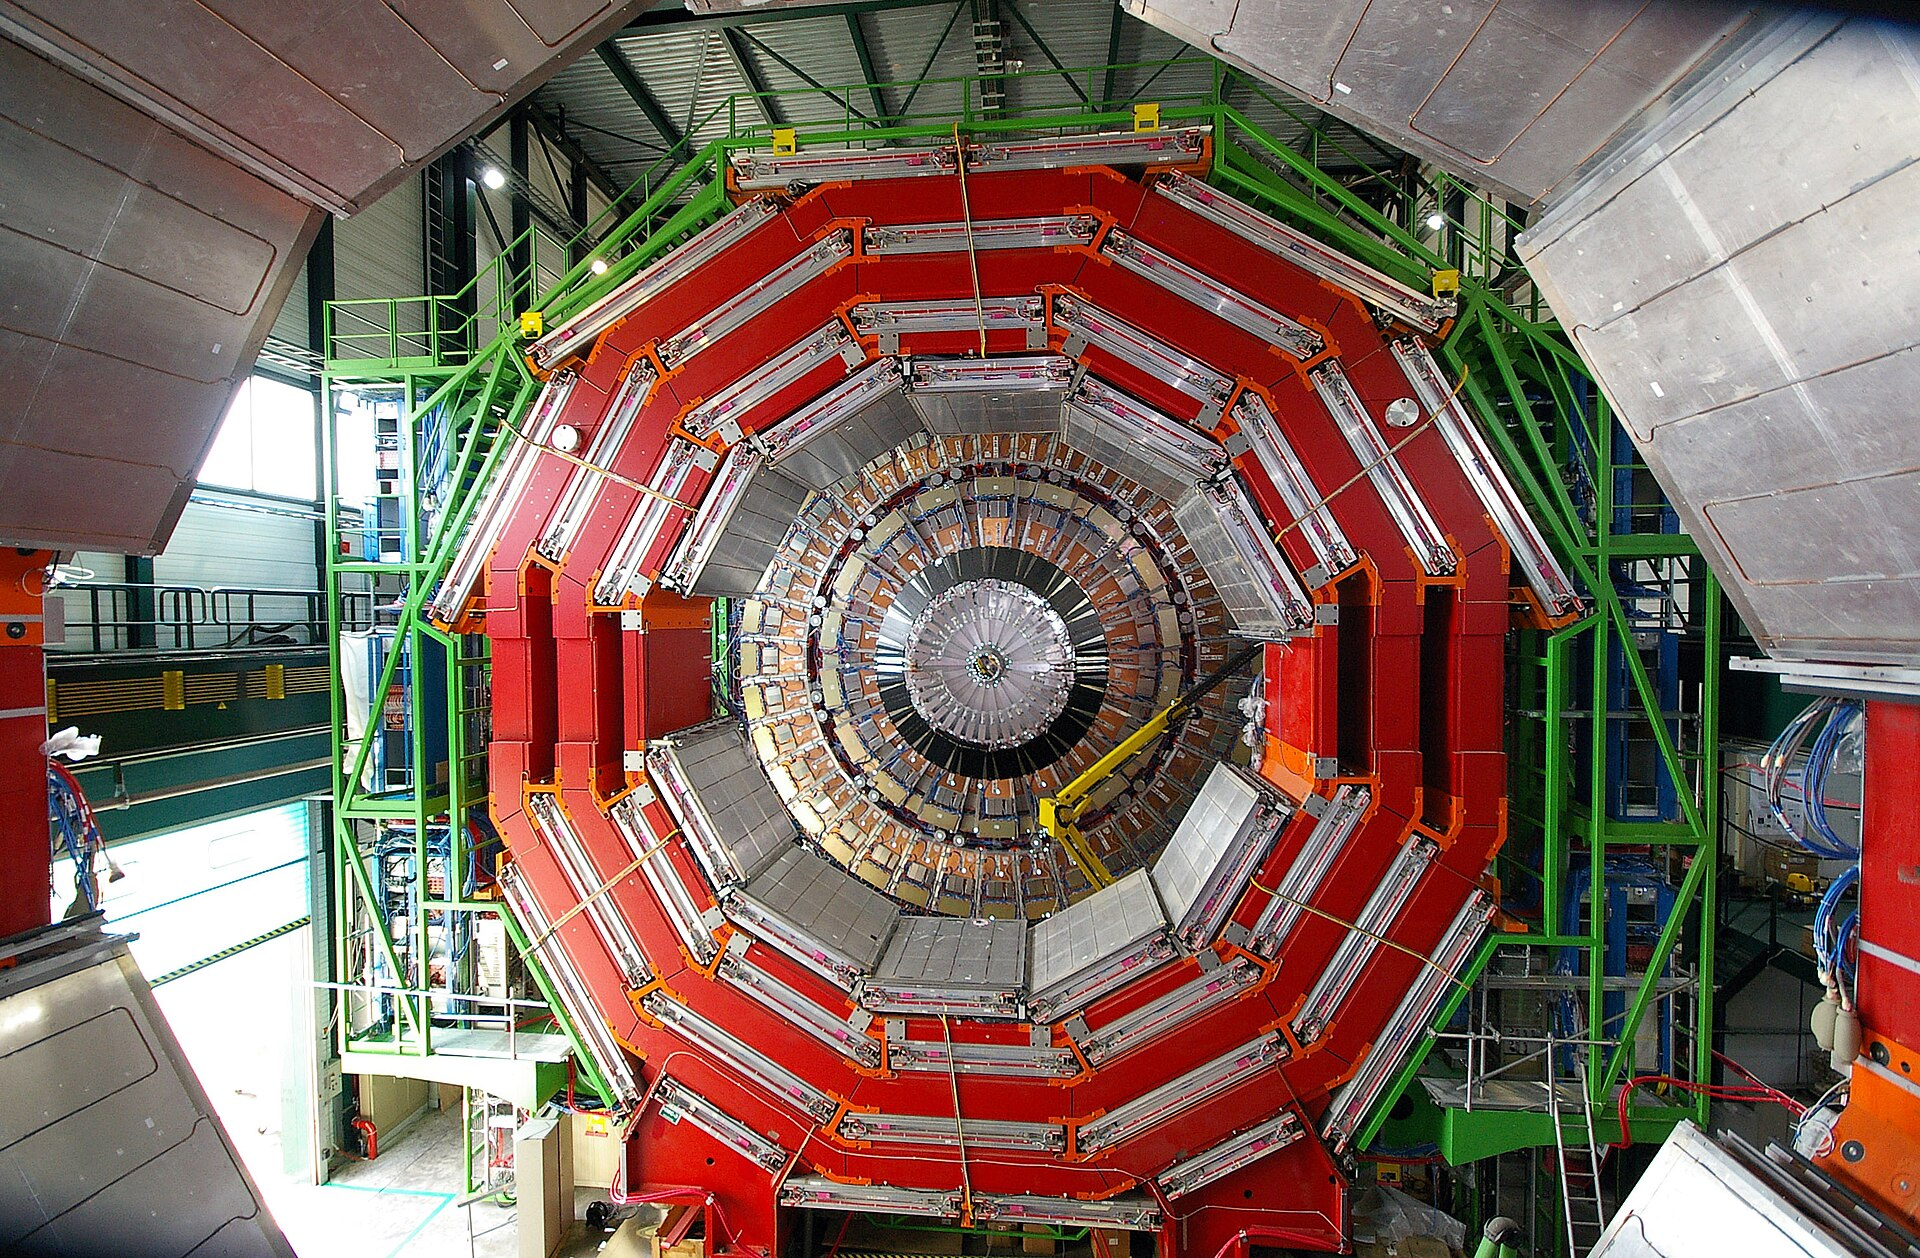
\includegraphics[width=0.62\linewidth]{images/book5/photo-cms-construction.jpg}

{\small निर्माणाधीन CMS संसूचक (छायाचित्र: जूलियन विलियम्स, मुक्त उपयोग): बंद होने से पहले, सामने से दिखती उसके ढोल की प्याज़-परतें --- इस अध्याय के अंतिम चित्र का पंद्रह हज़ार टन वाला क्रियान्वयन।}
\end{omfigure}

\section{समस्या: अटारी का म्यूऑन दूरदर्शी}

\begin{problem}\label{pb:b3:particle-physics:1}
\emph{अटारी का म्यूऑन दूरदर्शी।} विज्ञान मेले के लिए आप एक
ब्रह्मांडीय-किरण दूरदर्शी बनाते हैं: संदीप्तिकारक की दो
$20\times20$\,\unit{cm} तख्तियाँ, जिनमें एक दूसरी से \qty{30}{cm} ऊपर
हो, हर एक किसी प्रकाश-गुणक से पढ़ी जाए, और दोनों संपातिता में जुड़ी
हों --- यानी गिनती तभी जब \emph{दोनों} \qty{100}{ns} के भीतर चलें।
समुद्र-तल पर किसी क्षैतिज सतह से होकर म्यूऑन-अभिवाह:
प्रति \unit{cm^2} प्रति मिनट लगभग 1।

\medskip\noindent\textbf{भाग I --- आकाश को गिनना।}

\begin{enumerate}
  \item आपके म्यूऑन कहाँ शुरू होते हैं? शृंखला बताइए: आदिम
        प्रोटॉन, ऊपरी वायुमंडल, पायॉन, म्यूऑन --- और हर चरण पर कौन-सा
        बल राज करता है, यह भी।
  \item स्वयं पायॉन ज़मीन तक लगभग कभी क्यों नहीं पहुँचते
        ($\tau_\pi = \qty{26}{ns}$), जबकि उनकी संतान
        म्यूऑन पहुँच जाते हैं?
  \item दिए गए अभिवाह से अपनी एक-तख्ती दर की भविष्यवाणी कीजिए।
  \item अकेली तख्ती वस्तुतः कहीं अधिक बार चटकती है ---
        इलेक्ट्रॉनिकी का शोर और चारों ओर की रेडियोसक्रियता
        (\cref{ch:b3:nuclear-physics})। समझाइए कि
        दो-तख्ती संपातिता उसका लगभग सारा हिस्सा कैसे मार देती है।
  \item दो स्वतंत्र \qty{100}{Hz} शोर-स्रोत किसी \qty{100}{ns}
        खिड़की में कौन-सी आकस्मिक-संपातिता दर पैदा करते हैं
        ($R_{\text{आक}} = R_1R_2\Delta t$)? उसकी तुलना
        असली म्यूऑन-दर से कीजिए।
  \item आपकी संपातिता-दर प्रति मिनट 100 के पास ठहरती है ---
        जो एक-तख्ती वाली 400 से काफ़ी नीचे है। समझाइए: दो-तख्ती
        ज्यामिति किन म्यूऑनों को स्वीकारती है?
  \item दूरदर्शी को झुकाइए: दर नति-कोण के मोटे तौर पर
        $\cos^2\theta$ की तरह गिरती है। भौतिक कारण दीजिए
        ($\theta$ के साथ क्या बढ़ता है?)।
\end{enumerate}

\medskip\noindent\textbf{भाग II --- अटारी में सत्यापित आपेक्षिकता।}

\begin{enumerate}[resume]
  \item म्यूऑन: $\tau = \qty{2.2}{\micro s}$। $c\tau$ निकालिए और
        निष्कर्ष निकालिए कि \qty{15}{km} पर जन्मा कोई
        \emph{चिरसम्मत} म्यूऑन क्या कर पाता।
  \item आपके म्यूऑनों की औसत $E \approx \qty{4}{GeV}$ है
        ($m_\mu c^2 = \qty{106}{MeV}$): $\gamma$ निकालिए।
  \item फैला हुआ जीवनकाल, और उससे संगत परास: क्या अब अटारी की दर
        समझ में आती है?
  \item वही जीवित रहना म्यूऑन के तंत्र से फिर कहिए
        (\cref{ch:b3:relativistic-kinematics})।
  \item $\gamma = 38$ के लिए \qty{15}{km} से बचे रहने का अंश
        निकालिए ($t_{\text{निज}} = L/\gamma v$, बचाव
        $\eu^{-t/\tau}$)।
  \item अतः आपका दूरदर्शी \emph{कौन-सा} चिरसम्मत प्रयोग है, जो
        स्कूल के पुर्ज़ों से फिर बनाया गया? बताइए कि कोई शून्य
        परिणाम (चिरसम्मत क्षय) आपके गणक के लिए क्या भविष्यवाणी करता।
\end{enumerate}

\medskip\noindent\textbf{भाग III --- म्यूऑन है क्या।}

\begin{enumerate}[resume]
  \item म्यूऑन को मानक प्रतिरूप की मेज़ पर रखिए: कुल, पीढ़ी,
        आवेश, चक्रण।
  \item वह क्षय करता है: $\mu^- \to \text{e}^- + \bar\nu_{\text{e}} +
        \nu_\mu$। आवेश और दोनों \omterm{def:b3:particle-physics:zoo}{लेप्टॉन} कुल-संख्याएँ जाँचिए।
  \item क्षय-इलेक्ट्रॉन का ऊर्जा-वर्णक्रम सतत क्यों है,
        और उसका अंत-बिंदु क्या है ($\approx m_\mu c^2/2$)?
  \item $\mu^- \to \text{e}^- + \gamma$ --- जो कभी नहीं देखा गया
        --- आज के प्रयोगों के लिए इतना दिलचस्प क्यों है?
        (उसकी खोज क्या तोड़ देती?)
  \item आपकी तख्ती में रुककर विराम पर क्षय करता कोई म्यूऑन: उस
        विलंबित दूसरी कौंध का वर्णन कीजिए और यह भी कि वह आपको
        $\tau$ सीधे कैसे थमा देती है।
  \item म्यूऑन ``भारी इलेक्ट्रॉन'' हैं: परमाणुओं के लिए उसका एक
        परिणाम दीजिए --- किसी म्यूऑनी हाइड्रोजन की \omterm{thm:b3:hydrogen-atom:levels}{बोर
        त्रिज्या} का क्या होता है (\cref{ch:b3:hydrogen-atom}), जब
        उसे $m_\mu/m_{\text{e}} \approx 207$ से मापा जाए?
\end{enumerate}

\medskip\noindent\textbf{भाग IV --- शृंखला के ऊपर।}

\begin{enumerate}[resume]
  \item कोई $\qty{e15}{eV}$ आदिम प्रोटॉन लाखों कणों की झड़ी जगा
        देता है। यदि $10^{6}$ कण उसे बाँटें तो प्रति झड़ी-कण औसत
        ऊर्जा आकलिए।
  \item बड़ी वेधशालाएँ आपकी तख्तियों की जगह किलोमीटरों दूर रखे
        सैकड़ों जल-टैंक लगाती हैं, जो \emph{चेरेनकोव} प्रकाश
        ताकती हैं (\cref{pb:b3:nuclear-physics:1}):
        म्यूऑन उस पानी में क्या करते हैं, और टैंक \emph{दूर-दूर}
        क्यों?
  \item आपका संदीप्तिकारक-और-प्रकाश-गुणक वही सिद्धांत है जो बड़े
        संघट्टकों के कैलोरीमापियों का है:
        उस साझा सिद्धांत को एक वाक्य में बताइए
        (कण $\to$ प्रकाश $\to$ इलेक्ट्रॉन $\to$ गिनती)।
  \item कभी बुलबुला-कक्ष के छायाचित्र ही देखने का काम करते थे:
        किसी चुंबकीय क्षेत्र में कुंडली मारती आवेशित पगडंडियाँ। वह
        कुंडली आपको कौन-सी दो राशियाँ थमा देती है, और कौन-सा कण
        कोई पगडंडी छोड़ता ही नहीं?
  \item \cref{exo:b3:particle-physics:12} वाली रिकॉर्ड
        ब्रह्मांडीय किरण एक ही प्रोटॉन में किसी सर्व की गई टेनिस
        गेंद जितनी ऊर्जा लेकर टकराई। उसका होना
        प्रकृति के त्वरकों बनाम हमारे त्वरकों के बारे में क्या कहता है?
  \item मेले के पोस्टर का सार चार पंक्तियों में दीजिए: दस
        किलोमीटर ऊपर किसी प्रोटॉन से जन्मा, काल-विस्फार से पहुँचाया
        गया, दो संपाती कौंधों से पहचाना गया, और बारह कुर्सियों वाली
        एक मेज़ से समझाया गया।
\end{enumerate}
\end{problem}
